\documentclass[12pt,a4paper]{article}

\usepackage[utf8]{vietnam}
\usepackage{geometry}
\usepackage{graphicx}
\usepackage{amsmath}
\usepackage{amssymb}
\usepackage{float}
\usepackage{booktabs}
\usepackage{longtable}
\usepackage{array}
\usepackage{xcolor}
\usepackage{listings}
\usepackage{enumitem}
\usepackage{hyperref}
\usepackage{caption}
\usepackage{subcaption}

\geometry{left=2.8cm,right=2.2cm,top=2.5cm,bottom=2.5cm}
\hypersetup{
    colorlinks=true,
    linkcolor=blue,
    urlcolor=blue,
    citecolor=blue
}
\setlength{\parindent}{0pt}
\setlength{\parskip}{6pt}
\renewcommand{\arraystretch}{1.2}
\newcolumntype{P}[1]{>{\raggedright\arraybackslash}p{#1}}

\lstset{
    basicstyle=\ttfamily\small,
    breaklines=true,
    frame=single,
    columns=fullflexible,
    backgroundcolor=\color{gray!8}
}

\title{\textbf{BÁO CÁO ĐỒ ÁN}\\[0.4cm]
\Large Hệ thống định danh người dùng qua hành vi sử dụng điện thoại}
\author{
Môn học: Nhập môn Khoa học dữ liệu\\
Nhóm thực hiện: Nhóm đồ án NMKHDL
}
\date{Ngày biên soạn: 24/05/2026}

\begin{document}

\hypersetup{pageanchor=false}
\begin{titlepage}
    \centering
    {\Large \textbf{ĐẠI HỌC BÁCH KHOA HÀ NỘI}}\\
    {\large Trường Công nghệ Thông tin và Truyền thông}\\[2.0cm]

    {\LARGE \textbf{BÁO CÁO ĐỒ ÁN}}\\[0.6cm]
    {\Large \textbf{Hệ thống định danh người dùng qua hành vi sử dụng điện thoại}}\\[1.2cm]

    \begin{tabular}{rl}
        Môn học: & Nhập môn Khoa học dữ liệu \\
        Hướng tiếp cận: & Random Forest và CNN 1D \\
        Dữ liệu: & Hành vi cảm biến điện thoại và gõ phím \\
    \end{tabular}\\[1.6cm]

    \textbf{Thành viên nhóm}\\[0.3cm]
    \begin{tabular}{ll}
        Lương Mạnh Tường & 20225949 \\
        Bùi Minh Tuấn & 20225678 \\
        Trương Quốc Triệu & 20225941 \\
        Nguyễn Đức Thành & 20225930 \\
        Nguyễn Anh Tuấn & 20225772 \\
        Vũ Ngọc Lâm & 20225645 \\
        Vũ Nhật Quang & 20225761 \\
        Mai Văn Đăng & 20225699 \\
        Nguyễn Đình Thành & 20225670 \\
    \end{tabular}

    \vfill
    Hà Nội, 05/2026
\end{titlepage}

\hypersetup{pageanchor=true}
\pagenumbering{roman}
\tableofcontents
\newpage
\pagenumbering{arabic}

\section*{Tóm tắt}
\addcontentsline{toc}{section}{Tóm tắt}

Đồ án khảo sát bài toán định danh người dùng từ dữ liệu sử dụng điện thoại. Phần mô hình chính dùng tín hiệu cảm biến quán tính; log gõ phím được giữ như nguồn dữ liệu phụ để kiểm tra và mở rộng sau. Hai hướng được so sánh là Random Forest trên đặc trưng thủ công và CNN 1D trên chuỗi cảm biến. Với cách đánh giá 3-fold \textit{StratifiedGroupKFold}, Random Forest đạt macro-F1 trung bình 0.7845, cao hơn CNN 1D simple đạt 0.6881. Kết quả này cho thấy trong tập dữ liệu còn ít phiên ghi, đặc trưng thống kê được thiết kế thủ công vẫn là baseline mạnh và dễ giải thích.

\newpage

\section{Mô tả bài toán thực tế}

\subsection{Bối cảnh}

Điện thoại cá nhân thường chứa tài khoản, tin nhắn, ảnh và nhiều dữ liệu nhạy cảm. Mật khẩu, vân tay hoặc nhận diện khuôn mặt bảo vệ tốt ở thời điểm mở khoá, nhưng không theo dõi liên tục trong quá trình sử dụng. Sinh trắc học hành vi tiếp cận vấn đề từ một góc khác: nhận ra người dùng qua cách họ cầm, di chuyển và thao tác với thiết bị.

Trong đồ án này, hệ thống cần dự đoán người đang sử dụng điện thoại từ dữ liệu hành vi. Nguồn chính là chuyển động của điện thoại khi người dùng ngồi, đứng và đi bộ; dữ liệu gõ phím được dùng để ghi nhận thêm nhịp tương tác.

\subsection{Phát biểu bài toán}

Với mỗi mẫu dữ liệu cảm biến quán tính có dạng chuỗi thời gian:
\[
X_i \in \mathbb{R}^{128 \times 6}
\]
trong đó 128 là số mẫu trong một cửa sổ 2.56 giây, 6 kênh gồm \texttt{acc\_x, acc\_y, acc\_z, gyro\_x, gyro\_y, gyro\_z}. Mục tiêu là học hàm phân loại:
\[
f(X_i) \rightarrow y_i
\]
với \(y_i\) là mã người dùng trong tập người dùng đã biết.

Bài toán có hai chế độ đánh giá:

\begin{itemize}
    \item \textbf{Closed-set}: tất cả mẫu kiểm thử thuộc 12 người dùng đã xuất hiện trong huấn luyện.
    \item \textbf{Open-set}: một số người dùng chưa từng xuất hiện trong huấn luyện, hệ thống cần phát hiện tín hiệu ``người dùng chưa biết''.
\end{itemize}

\subsection{Ý nghĩa thực tế}

Nếu đạt độ tin cậy đủ cao, hướng này có thể dùng cho xác thực liên tục hoặc cảnh báo khi thiết bị có dấu hiệu bị người khác sử dụng. Trong đồ án, trọng tâm là xây dựng pipeline dữ liệu có thể chạy lại, chia train/validation đúng cách và giải thích rõ giới hạn của kết quả.

\section{Phương pháp học máy và dataset sử dụng}

\subsection{Dataset}

Bộ dữ liệu dùng trong báo cáo gồm 15 người dùng và 185 file CSV sau khi bỏ các log không dùng trong pipeline cuối. Các file còn lại được chia thành hai nhóm:

\begin{itemize}
    \item \textbf{Inertial}: dữ liệu cảm biến quán tính, gồm gia tốc kế và con quay hồi chuyển. Đây là nguồn dữ liệu chính dùng cho mô hình.
    \item \textbf{Keystroke}: dữ liệu gõ phím như thời điểm gõ, khoảng cách thời gian giữa các phím, tốc độ gõ.
\end{itemize}

Sau bước quét dữ liệu, \texttt{manifest.csv} được sinh ra để chuẩn hoá thông tin: người dùng, tên file, modality, hoạt động, session, attempt/rep, số dòng và tần số lấy mẫu ước lượng. Bảng \ref{tab:modality-counts} và \ref{tab:activity-counts} tóm tắt quy mô dữ liệu sau khi chuẩn hoá manifest.

\begin{table}[H]
    \centering
    \caption{Số lượng file theo modality}
    \label{tab:modality-counts}
    \begin{tabular}{lc}
        \toprule
        Modality & Số file \\
        \midrule
        Inertial & 154 \\
        Keystroke & 31 \\
        \midrule
        Tổng & 185 \\
        \bottomrule
    \end{tabular}
\end{table}

\begin{table}[H]
    \centering
    \caption{Số file inertial theo hoạt động}
    \label{tab:activity-counts}
    \begin{tabular}{lc}
        \toprule
        Hoạt động & Số file inertial \\
        \midrule
        sitting & 46 \\
        standing & 46 \\
        walking & 62 \\
        \bottomrule
    \end{tabular}
\end{table}

Mô hình chính dùng inertial vì đây là chuỗi thời gian liên tục và khớp trực tiếp với cả hai hướng mô hình: Random Forest trên đặc trưng thống kê và CNN 1D trên tín hiệu thô đã xử lý. Keystroke được trích đặc trưng trong \texttt{features.py} nhưng chưa đưa vào kết quả chính, để phần đánh giá tập trung vào một nguồn tín hiệu rõ ràng. Tần số lấy mẫu thực tế giữa các file không hoàn toàn đồng nhất, vì vậy pipeline có bước resample về 50 Hz trước khi chia cửa sổ.

\subsection{Tiền xử lý dữ liệu cảm biến}

Pipeline tiền xử lý được cài đặt trong \texttt{preprocess.py}. Các bước chính:

\begin{enumerate}
    \item Đọc dữ liệu cảm biến từ CSV.
    \item Điền giá trị thiếu bằng forward-fill/backward-fill.
    \item Resample về 50 Hz nếu tần số lấy mẫu thực tế lệch nhiều.
    \item Lọc low-pass Butterworth cutoff 20 Hz để giảm nhiễu cao tần.
    \item Lọc high-pass Butterworth cutoff 0.3 Hz cho ba trục gia tốc để tách thành phần trọng lực.
    \item Chia cửa sổ 128 mẫu, bước trượt 64 mẫu, tương đương overlap 50\%.
    \item Giới hạn tối đa 300 cửa sổ mỗi file để tránh một file dài chi phối toàn bộ tập huấn luyện.
\end{enumerate}

Kết quả lưu tại \texttt{windows.npz} với tensor:

\[
X \in \mathbb{R}^{39018 \times 128 \times 6}
\]

\subsection{Cách chia dữ liệu}

Sau tiền xử lý, tập inertial có 39018 cửa sổ, mỗi cửa sổ có kích thước \((128, 6)\). 15 người dùng trong dữ liệu gồm \texttt{userA}, \texttt{userB}, \texttt{userC}, \texttt{userD}, \texttt{userE}, \texttt{userF}, \texttt{userG}, \texttt{userH}, \texttt{userI}, \texttt{userK}, \texttt{userL}, \texttt{userM}, \texttt{userN}, \texttt{userP}, \texttt{userQ}. Nhóm chia dữ liệu theo hai tầng: tầng người dùng cho open-set và tầng file cho cross-validation closed-set.

\begin{table}[H]
    \centering
    \caption{Tách known/unknown ở mức người dùng}
    \label{tab:known-unknown}
    \begin{tabular}{lccc}
        \toprule
        Tập & Users & Windows & Groups/files \\
        \midrule
        Known closed-set & 12 & 29725 & 120 \\
        Unknown open-set & 3 & 9293 & 34 \\
        \midrule
        Tổng & 15 & 39018 & 154 \\
        \bottomrule
    \end{tabular}
\end{table}

Ba người dùng \texttt{userD}, \texttt{userE}, \texttt{userI} được giữ riêng cho bài toán open-set. Đây là chia tách ở mức user, không phải ở mức cửa sổ. Lý do là open-set cần mô phỏng đúng tình huống thực tế: hệ thống gặp một người dùng chưa từng xuất hiện trong giai đoạn huấn luyện. Nếu bất kỳ cửa sổ nào của các user unknown lọt vào train, bài toán sẽ không còn là open-set đúng nghĩa.

Với 12 user known còn lại, nhóm dùng \textit{StratifiedGroupKFold}. Điểm quan trọng là \textbf{không chia ngẫu nhiên theo cửa sổ}. Vì sliding window tạo ra nhiều cửa sổ liên tiếp, các cửa sổ gần nhau trong cùng một file có nội dung tín hiệu rất giống nhau. Nếu random split theo cửa sổ, train và validation có thể cùng chứa các đoạn gần như trùng từ một phiên ghi, làm mô hình học đặc trưng của phiên ghi thay vì học hành vi người dùng. Đây là dạng data leakage và thường làm điểm đánh giá cao giả tạo.

Để tránh leakage, mỗi cửa sổ được gắn group có dạng \texttt{user\_\_file}. Khi chia fold, toàn bộ cửa sổ sinh ra từ cùng một file luôn nằm trọn trong train hoặc trọn trong validation. Như vậy validation mô phỏng một phiên ghi mới hơn, khó hơn và gần thực tế hơn so với random split theo cửa sổ. Thành phần \textit{stratified} giúp phân phối user trong các fold tương đối cân bằng, còn \textit{group} đảm bảo ràng buộc không tách cùng một file sang hai tập. Tham số \texttt{shuffle=True, random\_state=42} được dùng để kết quả có thể tái lập.

Nhóm chọn 3-fold vì số file giữa các user không đều; user ít file nhất là \texttt{userQ}, chỉ có 3 file inertial. Nếu dùng 5-fold, một số fold validation có nguy cơ thiếu class, khiến macro-F1 không còn phản ánh đủ 12 user known. Với 3-fold, mỗi fold vẫn có đủ lớp để đánh giá ổn định hơn.

\begin{table}[H]
    \centering
    \caption{Thống kê train/validation của 3 fold closed-set}
    \label{tab:fold-split-stats}
    \begin{tabular}{lrrrr}
        \toprule
        Fold & Train windows & Val windows & Train groups & Val groups \\
        \midrule
        1 & 20069 & 9656 & 80 & 40 \\
        2 & 19814 & 9911 & 82 & 38 \\
        3 & 19567 & 10158 & 78 & 42 \\
        \bottomrule
    \end{tabular}
\end{table}

\subsection{Mô hình Random Forest}

Random Forest được dùng như baseline chính vì dễ giải thích và phù hợp với dữ liệu vừa/nhỏ. Mỗi cửa sổ cảm biến được chuyển thành vector 65 đặc trưng thủ công. Cấu trúc feature gồm \(6 \times 9 = 54\) đặc trưng thống kê/FFT cho 6 kênh, 9 đặc trưng correlation giữa các cặp trục được chọn, và 2 đặc trưng Signal Magnitude Area (SMA) cho accelerometer và gyroscope.

\begin{itemize}
    \item Thống kê theo từng trục: mean, standard deviation, MAD, min, max, IQR, energy.
    \item Đặc trưng miền tần số: FFT entropy, dominant frequency.
    \item Tương quan giữa các trục.
    \item Signal Magnitude Area cho accelerometer và gyroscope.
\end{itemize}

Mô hình sử dụng \texttt{RandomForestClassifier} với 300 cây. Tham số cân bằng lớp là \texttt{class\_weight=balanced\_subsample}. Random Forest phù hợp với bài toán này vì các đặc trưng thống kê và tần số tương đối ổn định khi số phiên ghi còn ít, mô hình ít tham số và không cần quá nhiều tinh chỉnh để đạt baseline tốt.

Để tránh leakage ở bước chuẩn hoá, \texttt{StandardScaler} chỉ được fit trên train fold. Sau đó scaler này mới được dùng để transform validation fold. Quy trình này đảm bảo validation không tham gia vào việc ước lượng trung bình và độ lệch chuẩn của đặc trưng.

\subsection{Mô hình CNN 1D}

CNN 1D được dùng để kiểm tra khả năng học trực tiếp từ chuỗi cảm biến. Sau khi đi qua \texttt{InertialDataset}, dữ liệu đầu vào có dạng \((B, 6, 128)\), trong đó \(B\) là batch size, 6 là số kênh cảm biến, 128 là chiều thời gian. Conv1D trượt kernel theo trục thời gian để học các mẫu biến thiên ngắn hạn của accelerometer và gyroscope.

\begin{lstlisting}
Input: (6, 128)
Conv1D(6 -> 32, kernel=7) + BatchNorm + ReLU + MaxPool
Conv1D(32 -> 64, kernel=5) + BatchNorm + ReLU + MaxPool
Conv1D(64 -> 128, kernel=3) + BatchNorm + ReLU
AdaptiveAvgPool1D
Dropout(0.3)
Linear(128 -> 12)
\end{lstlisting}

Trong kiến trúc này, BatchNorm giúp ổn định phân phối activation trong quá trình huấn luyện; ReLU tạo phi tuyến; MaxPool giảm chiều thời gian và giữ mẫu nổi bật; AdaptiveAvgPool gom toàn bộ chuỗi thành một vector cố định trước khi phân loại; Dropout giảm overfit. Kiến trúc được giữ ở mức 3 tầng convolution để báo cáo dễ giải thích và không biến phần mô hình thành một sweep phức tạp.

Cấu hình huấn luyện:

\begin{itemize}
    \item Optimizer: Adam.
    \item Learning rate: 0.001.
    \item Loss: CrossEntropy có class weight nghịch tần suất.
    \item Epoch: 40.
    \item Batch size: 128.
    \item Không dùng scheduler, không dùng MixUp/CutMix, không dùng sweep nhiều phase.
\end{itemize}

Việc không dùng scheduler hoặc augmentation phức tạp là lựa chọn có chủ đích cho bản báo cáo cuối: kết quả có thể thấp hơn một số thử nghiệm nâng cao, nhưng dễ tái lập, dễ trình bày và phù hợp hơn với đồ án nhập môn khoa học dữ liệu.

\subsection{Đánh giá open-set}

Với người dùng chưa biết, nhóm dùng hai cách tính điểm:

\begin{itemize}
    \item \textbf{Softmax max-prob}: nếu xác suất lớn nhất thấp, mẫu có khả năng thuộc unknown.
    \item \textbf{Mahalanobis}: đo khoảng cách embedding tới phân phối Gaussian của từng class đã biết.
\end{itemize}

Chỉ số dùng cho open-set là AUROC và TPR tại FPR = 5\%.

\section{Kết quả thí nghiệm đánh giá hiệu năng}

\subsection{Chỉ số đánh giá}

Nhóm sử dụng nhiều chỉ số vì mỗi chỉ số phản ánh một khía cạnh khác nhau của hệ thống:

\begin{itemize}
    \item \textbf{Accuracy}: tỷ lệ dự đoán đúng trên toàn bộ mẫu. Chỉ số này dễ hiểu, nhưng có thể bị ảnh hưởng khi số cửa sổ giữa các user không đều.
    \item \textbf{Macro-F1}: tính F1 riêng cho từng user rồi lấy trung bình. Chỉ số này phù hợp hơn cho bài toán định danh nhiều người dùng vì mỗi user có trọng số như nhau trong điểm cuối.
    \item \textbf{AUROC}: dùng cho open-set, đánh giá khả năng phân biệt known và unknown khi thay đổi ngưỡng quyết định.
    \item \textbf{TPR@FPR=5\%}: mô phỏng yêu cầu bảo mật, chỉ cho phép tỷ lệ nhận nhầm unknown thành known ở mức thấp.
\end{itemize}

Với \(C\) class người dùng, macro-F1 được tính theo:

\[
MacroF1 = \frac{1}{C}\sum_{c=1}^{C} F1_c
\]

\subsection{Kết quả tổng thể}

Kết quả được chạy lại với cấu hình đơn giản, lưu tại \texttt{simple\_results.json}. Bảng \ref{tab:main-results} trình bày điểm trung bình trên 3 fold.

\begin{table}[H]
    \centering
    \caption{Kết quả closed-set theo 3-fold StratifiedGroupKFold}
    \label{tab:main-results}
    \begin{tabular}{lccc}
        \toprule
        Mô hình & Macro-F1 trung bình & Độ lệch chuẩn & Accuracy trung bình \\
        \midrule
        CNN 1D simple & 0.6881 & 0.0077 & -- \\
        Random Forest & \textbf{0.7845} & 0.0204 & \textbf{0.8013} \\
        \bottomrule
    \end{tabular}
\end{table}

\begin{figure}[H]
    \centering
    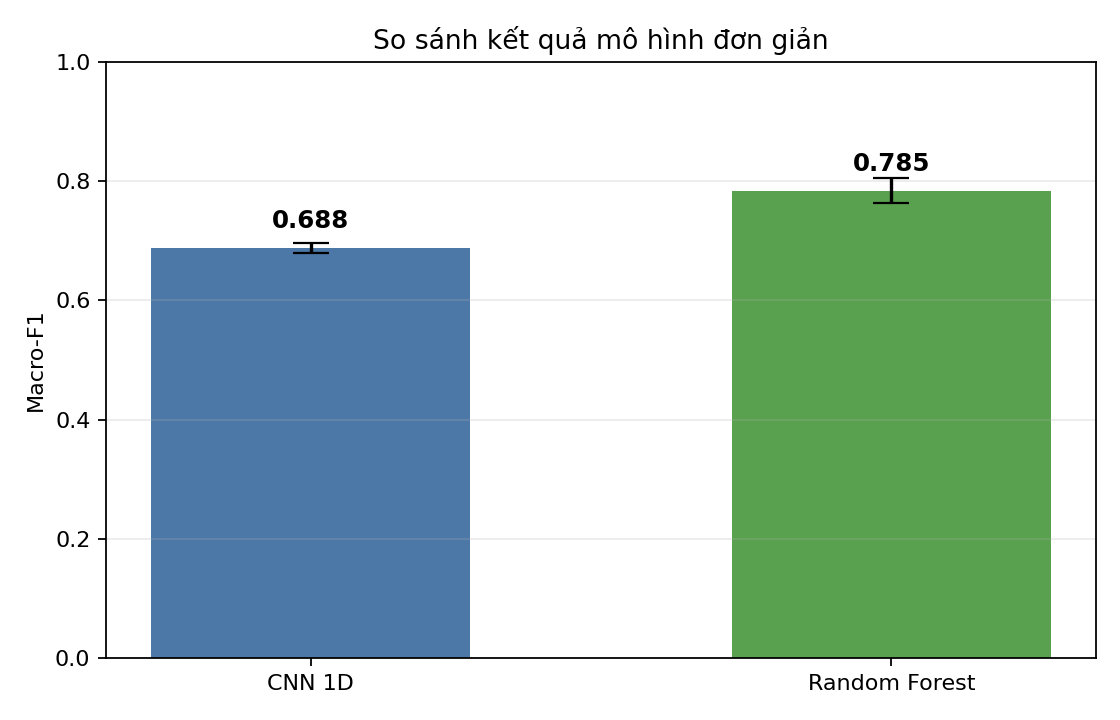
\includegraphics[width=0.78\textwidth]{figures/simple_model_comparison.png}
    \caption{So sánh macro-F1 giữa CNN 1D và Random Forest}
    \label{fig:model-comparison}
\end{figure}

Random Forest đạt \(0.7845 \pm 0.0204\) macro-F1 và accuracy trung bình 0.8013. CNN 1D simple đạt \(0.6881 \pm 0.0077\) macro-F1. Như vậy RF cao hơn CNN khoảng 0.0964 macro-F1. Kết quả này không có nghĩa là CNN là mô hình kém, mà cho thấy dữ liệu hiện tại chưa đủ lớn và chưa đủ đa phiên để CNN phát huy hết khả năng học đặc trưng tự động. Trong khi đó, feature thống kê thủ công của RF đã mã hoá trực tiếp nhiều thông tin hữu ích về biên độ, năng lượng, tần số và tương quan giữa các trục.

Đây là một kết luận quan trọng của đồ án: với dữ liệu chưa lớn, số phiên ghi của mỗi người chưa nhiều, đặc trưng thống kê thủ công kết hợp với mô hình cây vẫn rất cạnh tranh. Vì vậy báo cáo chọn Random Forest là mô hình chính và CNN 1D là mô hình học sâu bổ sung.

\subsection{Độ ổn định theo fold}

\begin{table}[H]
    \centering
    \caption{Macro-F1 trên từng fold}
    \label{tab:fold-results}
    \begin{tabular}{lccc}
        \toprule
        Mô hình & Fold 1 & Fold 2 & Fold 3 \\
        \midrule
        CNN 1D simple & 0.6933 & 0.6772 & 0.6938 \\
        Random Forest & 0.7876 & 0.7582 & 0.8077 \\
        \bottomrule
    \end{tabular}
\end{table}

\begin{figure}[H]
    \centering
    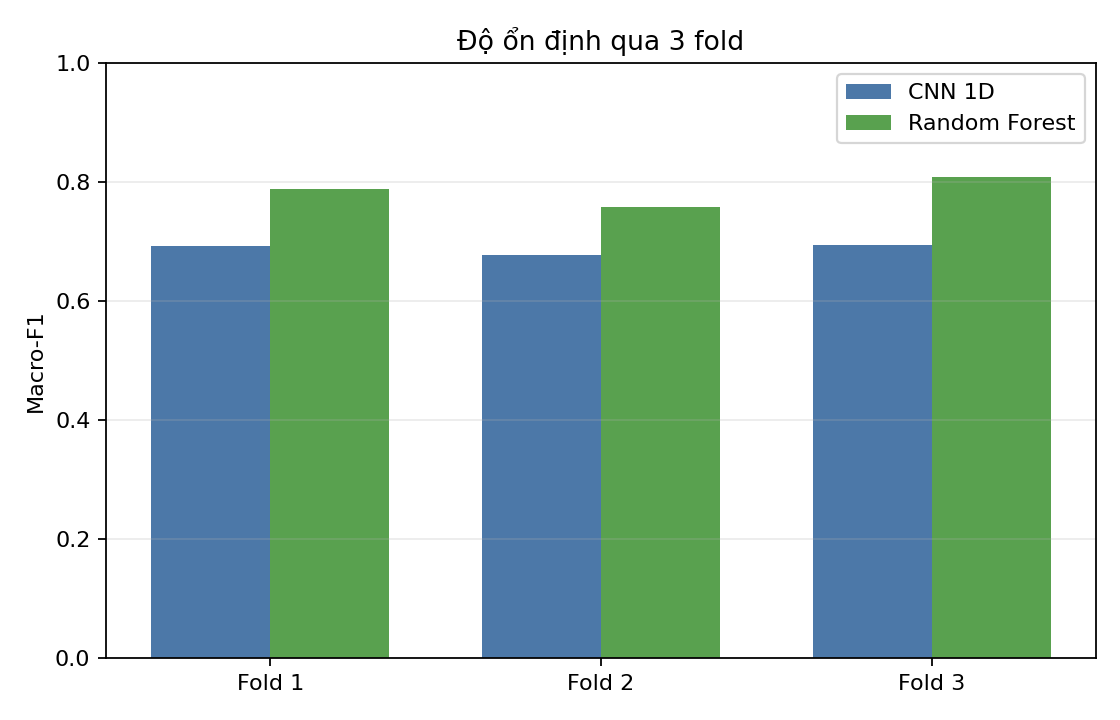
\includegraphics[width=0.78\textwidth]{figures/simple_fold_macro_f1.png}
    \caption{Macro-F1 của từng mô hình qua 3 fold}
    \label{fig:fold-f1}
\end{figure}

CNN có độ lệch chuẩn nhỏ hơn, tức kết quả giữa các fold ổn định hơn, nhưng mức điểm trung bình thấp hơn. Random Forest dao động nhiều hơn một chút giữa các fold nhưng vẫn là mô hình có hiệu năng tốt nhất. Điều này phù hợp với trực giác: RF tận dụng feature thủ công tốt hơn trong dữ liệu nhỏ, còn CNN cần thêm dữ liệu hoặc thêm phiên ghi để học biểu diễn bền vững hơn.

\subsection{Accuracy của Random Forest}

\begin{figure}[H]
    \centering
    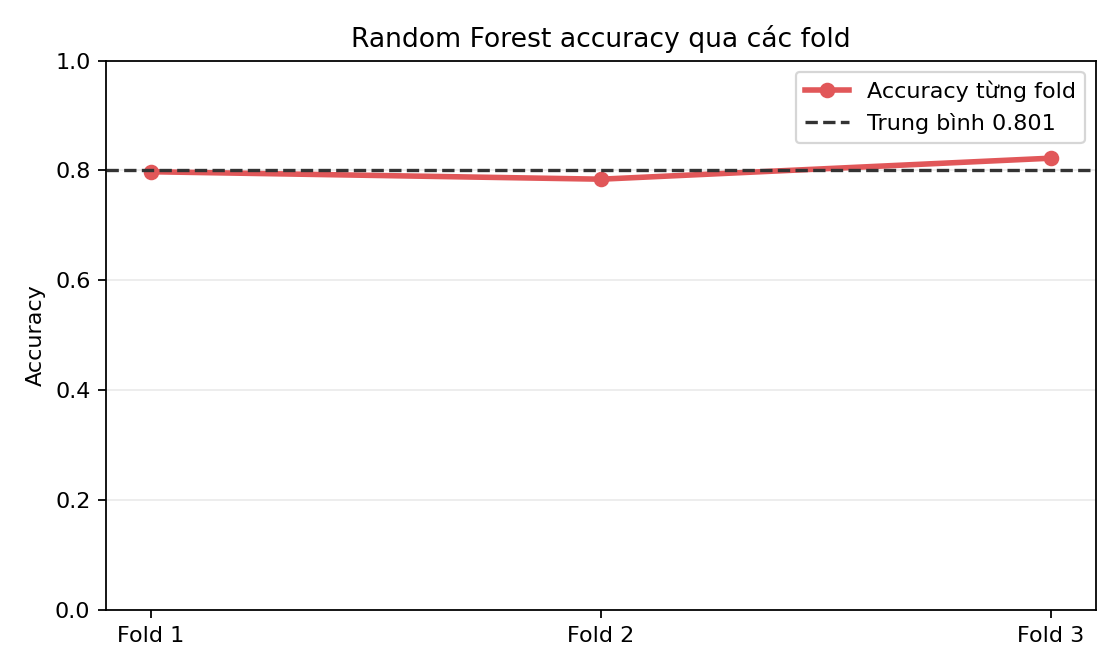
\includegraphics[width=0.78\textwidth]{figures/simple_rf_accuracy.png}
    \caption{Accuracy của Random Forest qua từng fold}
    \label{fig:rf-accuracy}
\end{figure}

Accuracy trung bình của Random Forest đạt 0.8013. Chỉ số này dễ hiểu với người nghe không chuyên, còn macro-F1 được ưu tiên trong đánh giá chính vì dữ liệu giữa các người dùng không hoàn toàn cân bằng.

\subsection{Phân tích CNN theo hoạt động}

Kết quả cũ của pipeline đánh giá tổng hợp cũng tạo được biểu đồ theo hoạt động và ma trận nhầm lẫn. Hai hình này dùng để phân tích sâu hơn các lỗi của mô hình CNN.

\begin{figure}[H]
    \centering
    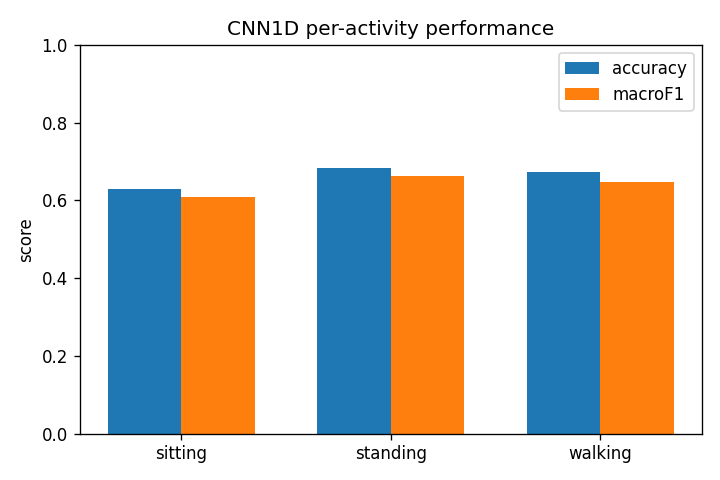
\includegraphics[width=0.72\textwidth]{figures/cnn_per_activity.png}
    \caption{Hiệu năng CNN theo hoạt động sitting, standing, walking}
    \label{fig:per-activity}
\end{figure}

\begin{figure}[H]
    \centering
    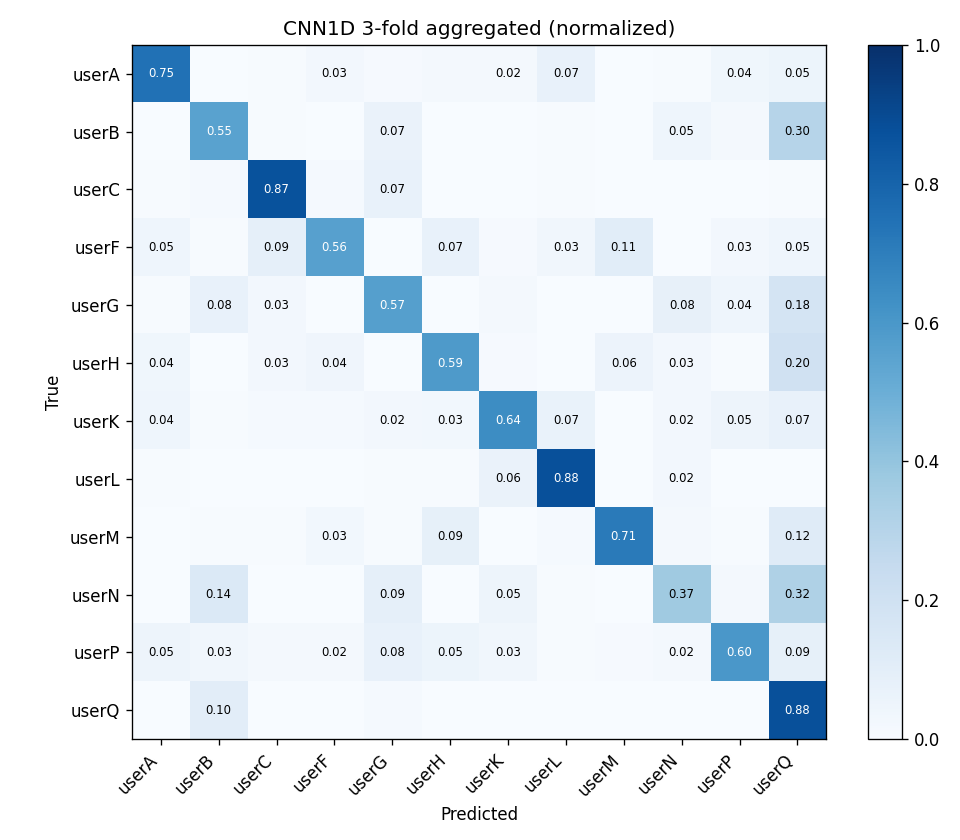
\includegraphics[width=0.82\textwidth]{figures/cnn_confusion.png}
    \caption{Ma trận nhầm lẫn chuẩn hoá của CNN}
    \label{fig:confusion}
\end{figure}

\subsection{Kết quả open-set}

\begin{table}[H]
    \centering
    \caption{Kết quả phát hiện người dùng chưa biết}
    \label{tab:openset}
    \begin{tabular}{lcc}
        \toprule
        Phương pháp & AUROC trung bình & TPR @ FPR = 5\% \\
        \midrule
        Softmax max-prob & \textbf{0.6702} & \textbf{0.2782} \\
        Mahalanobis & 0.6124 & 0.0807 \\
        \bottomrule
    \end{tabular}
\end{table}

Open-set chưa phải điểm mạnh của hệ thống hiện tại. Softmax max-prob đạt AUROC 0.6702, tốt hơn Mahalanobis nhưng vẫn chỉ nên xem là baseline. AUROC khoảng 0.67 cho thấy có tín hiệu phân biệt known/unknown, nhưng chưa đủ tốt để triển khai thực tế. Nguyên nhân chính là embedding học từ dữ liệu nhỏ chưa tạo biên phân tách đủ ổn định, đặc biệt khi số phiên ghi mỗi user còn hạn chế.

\section{Các chức năng chính của hệ thống và cách sử dụng}

\subsection{Chức năng chính}

Hệ thống được tổ chức thành các bước độc lập, có thể chạy lại từng phần.

\begin{longtable}{P{0.08\textwidth}P{0.37\textwidth}P{0.39\textwidth}}
\caption{Các chức năng chính của hệ thống} \\
\toprule
STT & Lệnh & Chức năng \\
\midrule
\endfirsthead
\toprule
STT & Lệnh & Chức năng \\
\midrule
\endhead
1 & \path{python -m src.io} & Quét dữ liệu thô, parse tên file, sinh \texttt{manifest.csv}. \\
2 & \path{python -m src.preprocess} & Tiền xử lý cảm biến, lọc tín hiệu, chia cửa sổ, sinh \texttt{windows.npz}. \\
3 & \path{python -m src.features} & Trích đặc trưng gõ phím phục vụ phân tích bổ sung. \\
4 & \path{python -m scripts.run_simple_pipeline} & Chạy pipeline đơn giản gồm CNN 1D và RF, lưu \texttt{simple\_results.json}. \\
5 & \path{python -m scripts.plot_simple_results} & Vẽ biểu đồ so sánh mô hình, fold và accuracy. \\
6 & \path{python -m src.openset} & Đánh giá phát hiện user unknown bằng softmax/Mahalanobis. \\
7 & \path{jupyter lab simple_pipeline.ipynb} & Chạy notebook minh hoạ kết quả và biểu đồ trong JupyterLab. \\
\bottomrule
\end{longtable}

\subsection{Cài đặt môi trường}

Yêu cầu Python 3.10 trở lên. Các gói chính được liệt kê trong \texttt{requirements.txt}: \texttt{numpy}, \texttt{pandas}, \texttt{scipy}, \texttt{scikit-learn}, \texttt{torch}, \texttt{matplotlib}, \texttt{seaborn}, \texttt{joblib}, \texttt{tqdm}, \texttt{jupyterlab}.

\begin{lstlisting}[language=bash]
python3 -m venv venv
source venv/bin/activate
pip install -r requirements.txt --index-url https://pypi.org/simple
\end{lstlisting}

\subsection{Chạy pipeline đơn giản}

\begin{lstlisting}[language=bash]
source venv/bin/activate
python -m scripts.run_simple_pipeline
python -m scripts.plot_simple_results
\end{lstlisting}

Kết quả chính:

\begin{itemize}
    \item \texttt{simple\_results.json}: điểm số CNN và RF.
    \item \texttt{simple\_model\_comparison.png}: so sánh tổng thể.
    \item \texttt{simple\_fold\_macro\_f1.png}: điểm từng fold.
    \item \texttt{simple\_rf\_accuracy.png}: accuracy của RF.
\end{itemize}

\subsection{Chạy bằng JupyterLab}

Nhóm đã chuẩn bị notebook \texttt{simple\_pipeline.ipynb}. Mở notebook bằng:

\begin{lstlisting}[language=bash]
source venv/bin/activate
jupyter lab simple_pipeline.ipynb
\end{lstlisting}

Trong notebook, biến \texttt{RUN\_TRAIN} mặc định là \texttt{False} để không train lại CNN mỗi lần mở. Nếu muốn chạy lại toàn bộ, đổi \texttt{RUN\_TRAIN = True}. Nếu chỉ muốn cập nhật RF và biểu đồ, đổi \texttt{RUN\_RF\_ONLY = True}.

\section{Cấu trúc mã nguồn và vai trò các class/method chính}

\subsection{Tổ chức mã nguồn}

Mã nguồn được tách theo đúng luồng xử lý: đọc dữ liệu, tiền xử lý, định nghĩa dataset, huấn luyện, đánh giá và vẽ hình. Trong báo cáo chỉ nêu tên file chính để tránh làm phần trình bày bị nặng bởi đường dẫn thư mục.

\subsection{Vai trò các module chính}

\begin{longtable}{P{0.34\textwidth}P{0.56\textwidth}}
\caption{Vai trò các module chính} \\
\toprule
File & Vai trò \\
\midrule
\endfirsthead
\toprule
File & Vai trò \\
\midrule
\endhead
\texttt{config.py} & Khai báo đường dẫn, kích thước cửa sổ, danh sách kênh cảm biến, user unknown, seed. \\
\texttt{io.py} & Parse tên file, đọc CSV, ước lượng tần số lấy mẫu, xây dựng manifest. \\
\texttt{preprocess.py} & Resample, lọc Butterworth, tách trọng lực, chia sliding window. \\
\texttt{features.py} & Trích đặc trưng thống kê, FFT, correlation, SMA và đặc trưng keystroke. \\
\texttt{datasets.py} & Định nghĩa \texttt{InertialDataset}, chuẩn hoá dữ liệu, chuyển shape cho Conv1D. \\
\texttt{models.py} & Định nghĩa \texttt{CNN1D} và factory \texttt{make\_model}. \\
\texttt{train.py} & Chạy huấn luyện 3-fold, lưu checkpoint và log experiment. \\
\texttt{evaluate.py} & Chạy Random Forest baseline, gom prediction CNN, vẽ confusion/per-activity. \\
\texttt{openset.py} & Đánh giá softmax max-prob và Mahalanobis cho open-set. \\
\texttt{run\_simple\_pipeline.py} & Script đơn giản hoá để chạy đúng hai mô hình chính: CNN 1D và RF. \\
\texttt{plot\_simple\_results.py} & Tạo ba biểu đồ chính dùng trong báo cáo. \\
\bottomrule
\end{longtable}

\subsection{Class và method quan trọng}

\begin{itemize}
    \item \texttt{InertialDataset.\_\_getitem\_\_}: lấy một cửa sổ cảm biến, chuẩn hoá theo mean/std của train fold, chuyển từ shape \((T, C)\) sang \((C, T)\) cho PyTorch Conv1D.
    \item \texttt{CNN1D.forward}: chạy chuỗi Conv1D, BatchNorm, ReLU, pooling và linear head để dự đoán người dùng.
    \item \texttt{CNN1D.embed}: trả embedding trước lớp phân loại, dùng cho open-set.
    \item \texttt{run\_cv}: thực hiện vòng lặp 3-fold, gọi train từng fold, lưu checkpoint và metric.
    \item \texttt{rf\_baseline}: trích đặc trưng thủ công, chuẩn hoá, train Random Forest và tính macro-F1/accuracy.
    \item \texttt{plot\_model\_comparison}, \texttt{plot\_fold\_scores}, \texttt{plot\_rf\_accuracy}: sinh hình minh hoạ kết quả.
\end{itemize}

\section{Khó khăn gặp phải và cách giải quyết}

\subsection{Tên file và schema dữ liệu không đồng nhất}

Các file dữ liệu có nhiều quy ước đặt tên khác nhau, ví dụ \texttt{\_s1\_att2.csv}, \texttt{\_s1\_r3.csv}, hoặc thiếu một số thành phần. Nếu parse thủ công từng trường hợp, pipeline dễ lỗi và khó mở rộng. Nhóm xử lý bằng các regex riêng trong \texttt{io.py}, sau đó sinh manifest thống nhất.

\subsection{Nguy cơ rò rỉ dữ liệu khi chia train/validation}

Nếu chia ngẫu nhiên theo cửa sổ, các cửa sổ từ cùng một file có thể xuất hiện ở cả train và validation. Do cửa sổ trượt có overlap 50\%, nhiều mẫu liền kề gần như cùng biểu diễn một đoạn chuyển động. Điều này làm điểm số tăng giả tạo vì mô hình học đặc trưng riêng của phiên ghi thay vì học hành vi người dùng. Giải pháp là dùng \textit{StratifiedGroupKFold} theo group \texttt{user\_\_file}, đảm bảo cùng một file không bị tách sang hai tập.

\subsection{Ít file ở một số người dùng}

Số file inertial giữa các user không đều. User ít nhất là \texttt{userQ}, chỉ có 3 file inertial. Nếu cố dùng 5-fold, một số fold validation có thể thiếu user này, làm macro-F1 không đánh giá đủ class và khiến kết quả kém tin cậy. Giải pháp là chọn 3-fold, cân bằng giữa số lần đánh giá và điều kiện mỗi fold vẫn có đủ 12 user known.

\subsection{Mất cân bằng số cửa sổ giữa các file}

Một số file dài sinh ra rất nhiều cửa sổ, khiến một vài người dùng hoặc phiên ghi chi phối dữ liệu huấn luyện. Giải pháp là giới hạn tối đa 300 cửa sổ mỗi file và lấy mẫu đều theo thời gian bằng \texttt{np.linspace}.

\subsection{Dữ liệu cảm biến có nhiễu và khác tần số}

Dữ liệu thực tế từ điện thoại có thể lệch tần số lấy mẫu hoặc nhiễu cao tần. Pipeline xử lý bằng cách resample về 50 Hz, low-pass 20 Hz và high-pass 0.3 Hz cho gia tốc.

\subsection{CNN không vượt Random Forest}

Ban đầu kỳ vọng CNN 1D sẽ tốt hơn do học trực tiếp từ chuỗi cảm biến. Tuy nhiên, kết quả simple cho thấy Random Forest đạt macro-F1 0.7845, cao hơn CNN 0.6881. Nhóm chọn báo cáo trung thực kết quả này và lý giải rằng với dữ liệu nhỏ, đặc trưng thủ công vẫn hiệu quả hơn mô hình học sâu.

\subsection{Open-set còn yếu}

AUROC open-set chỉ đạt khoảng 0.67 với softmax max-prob. Nguyên nhân là embedding chưa đủ ổn định khi số phiên/người còn ít. Giải pháp đề xuất là tăng số phiên ghi, thu thêm dữ liệu unknown và thử các phương pháp học biểu diễn như contrastive learning ở giai đoạn sau.

\subsection{Tái lập thí nghiệm open-set}

Khi rà soát lại thí nghiệm, nhóm nhận thấy phần open-set phải tự tách known/unknown trong \texttt{openset.py}. Nếu dùng lại helper của closed-set, script có nguy cơ chỉ đọc phần known và không đánh giá đúng các user unknown. Phiên bản hiện tại tạo mask theo \texttt{UNKNOWN\_USERS}, đồng thời đọc được cả checkpoint cũ và mới. Nhờ vậy lệnh \texttt{python -m src.openset} có thể chạy lại để sinh \texttt{openset\_results.json}.

\section{Khám phá mới hoặc kết luận}

\subsection{Khám phá chính}

\begin{enumerate}
    \item \textbf{Random Forest là lựa chọn phù hợp nhất cho báo cáo chính}. Mô hình này đạt điểm cao hơn CNN, dễ giải thích hơn và ít tham số lạ với người mới học khoa học dữ liệu.
    \item \textbf{Đánh giá group-by-file là bắt buộc}. Nếu không nhóm theo file, kết quả có thể bị leakage và không phản ánh khả năng tổng quát hoá tới phiên ghi mới.
    \item \textbf{Dữ liệu chuyển động giàu thông tin hơn khi hoạt động có chuyển động rõ}. Các hoạt động như walking/standing thường cho tín hiệu phân biệt người dùng tốt hơn sitting.
    \item \textbf{Deep learning không phải lúc nào cũng thắng}. Trong bối cảnh dữ liệu nhỏ, mô hình cổ điển với feature tốt có thể vượt mô hình CNN đơn giản.
    \item \textbf{Open-set cần thêm dữ liệu và phương pháp chuyên biệt}. Softmax max-prob chỉ là baseline, chưa đủ tốt cho triển khai thực tế.
\end{enumerate}

\subsection{Kết luận}

Đồ án đã hoàn thành pipeline từ dữ liệu thô tới đánh giá mô hình: đọc CSV, chuẩn hoá manifest, tiền xử lý cảm biến, chia cửa sổ, trích đặc trưng, huấn luyện Random Forest và CNN 1D, đánh giá closed-set/open-set và sinh biểu đồ báo cáo.

Với yêu cầu của môn học, hướng trình bày nên tập trung vào hai mô hình:

\begin{itemize}
    \item Random Forest: mô hình chính, đạt macro-F1 0.7845 và accuracy 0.8013.
    \item CNN 1D: mô hình học sâu bổ sung, đạt macro-F1 0.6881.
\end{itemize}

Các thử nghiệm phức tạp như ResNet, TCN, BiLSTM, scheduler, MixUp/CutMix không nên đưa vào phần chính vì làm báo cáo khó theo dõi. Chúng có thể được xem là hướng thử nghiệm phụ nếu cần mở rộng.

\subsection{Hướng phát triển}

\begin{itemize}
    \item Thu thêm dữ liệu nhiều phiên hơn cho mỗi người dùng.
    \item Kết hợp inertial với keystroke ở mức feature fusion.
    \item Cải thiện open-set bằng threshold calibration hoặc học biểu diễn tương phản.
    \item Tạo giao diện demo đơn giản để upload CSV và dự đoán người dùng.
\end{itemize}

\subsection{Đóng gói sản phẩm nộp}

Theo yêu cầu nộp đồ án, sản phẩm cuối nên được đóng gói thành một file nén chứa đầy đủ mã nguồn, hướng dẫn chạy và báo cáo. Các thành phần cần có:

\begin{itemize}
    \item Mã nguồn dự án và cấu hình thí nghiệm.
    \item Hướng dẫn cài đặt và chạy: \texttt{README.md} và \texttt{requirements.txt}.
    \item Báo cáo cuối: \texttt{bao\_cao.pdf}.
    \item Notebook minh hoạ: \texttt{simple\_pipeline.ipynb}.
    \item Kết quả số: \texttt{simple\_results.json}.
    \item Các hình kết quả dùng trong báo cáo.
\end{itemize}

Khi nộp, nên kiểm tra lại rằng người chấm có thể đọc \texttt{README.md}, cài môi trường bằng \texttt{requirements.txt}, chạy pipeline đơn giản, mở notebook và xem được báo cáo PDF mà không cần tái tạo toàn bộ các thử nghiệm cũ.

\section*{Phụ lục: Lệnh biên dịch báo cáo}
\addcontentsline{toc}{section}{Phụ lục: Lệnh biên dịch báo cáo}

Trong thư mục chứa \texttt{bao\_cao.tex}, chạy:

\begin{lstlisting}[language=bash]
pdflatex bao_cao.tex
pdflatex bao_cao.tex
\end{lstlisting}

File PDF đầu ra là \texttt{bao\_cao.pdf}.

\begin{thebibliography}{9}
\bibitem{sklearn}
Pedregosa et al., \textit{Scikit-learn: Machine Learning in Python}, Journal of Machine Learning Research, 2011.

\bibitem{pytorch}
Paszke et al., \textit{PyTorch: An Imperative Style, High-Performance Deep Learning Library}, NeurIPS, 2019.

\bibitem{scipy}
Virtanen et al., \textit{SciPy 1.0: Fundamental Algorithms for Scientific Computing in Python}, Nature Methods, 2020.

\bibitem{uci-har}
Anguita et al., \textit{A Public Domain Dataset for Human Activity Recognition Using Smartphones}, ESANN, 2013.
\end{thebibliography}

\end{document}
